\def\SECTION{3.2 Parallel Lines and Transversals}
\documentclass[aspectratio=169,14pt]{beamer}
\usepackage[T1]{fontenc}
\usepackage{mathpazo}
\usepackage{amsmath,amssymb}
\usepackage{tikz}
\usetikzlibrary{arrows.meta,calc,decorations.pathreplacing}
\definecolor{fblue}{HTML}{1F4E79}
\definecolor{fteal}{HTML}{0F7C7C}
\definecolor{fgold}{HTML}{C9962B}
\definecolor{fred}{HTML}{B3261E}
\definecolor{fink}{HTML}{16233B}
\definecolor{fsoft}{HTML}{EEF3F8}
\definecolor{fgoldsoft}{HTML}{FBF1DC}
\setbeamertemplate{navigation symbols}{}
\setbeamercolor{normal text}{fg=fink}
\setbeamercolor{frametitle}{fg=fblue}
\setbeamerfont{frametitle}{series=\bfseries,size=\Large}
\setbeamercolor{structure}{fg=fteal}
\setbeamertemplate{itemize item}{\color{fteal}$\blacktriangleright$}
\setbeamertemplate{frametitle}{\vspace{6pt}\insertframetitle\par\vspace{-2pt}{\color{fgold}\rule{2.2cm}{2pt}}}
\setbeamertemplate{footline}{\hspace{0.6cm}{\color{fblue}\scriptsize\bfseries Fang\textcolor{fteal}{Math}}\hfill{\scriptsize\color{gray}\SECTION\quad\insertframenumber}\hspace{0.6cm}\vspace{6pt}}
\newcommand{\key}[1]{{\color{fteal}\textbf{#1}}}
\newcommand{\ans}[1]{\colorbox{fgoldsoft}{\color{fink}\ensuremath{#1}}}
\newcommand{\warn}[1]{\begin{beamercolorbox}[sep=8pt,rounded=true]{warnbox}{\color{fred}\textbf{Watch out!}}\enskip #1\end{beamercolorbox}}
\setbeamercolor{warnbox}{bg=fred!8,fg=fink}
\setbeamercolor{turnbox}{bg=fgoldsoft,fg=fink}
\setbeamercolor{defbox}{bg=fsoft,fg=fink}
\newcommand{\defn}[1]{\begin{beamercolorbox}[sep=8pt,rounded=true]{defbox}#1\end{beamercolorbox}}
\newenvironment{yourturn}{\begin{beamercolorbox}[sep=10pt,rounded=true]{turnbox}{\color{fgold}\Large\bfseries Your turn!}\quad{\small Pause the video and try it.}\par\medskip}{\end{beamercolorbox}}
\newcommand{\titleframe}[3]{%
\begin{frame}[plain]
\begin{tikzpicture}[remember picture,overlay]
\fill[fblue] (current page.north west) rectangle ([yshift=-0.9cm]current page.north east);
\node[anchor=west,text=white,font=\bfseries] at ([xshift=0.6cm,yshift=-0.45cm]current page.north west) {Fang\textcolor{fgold}{Math}};
\node[anchor=east,text=white,font=\small] at ([xshift=-0.6cm,yshift=-0.45cm]current page.north east) {Geometry $\cdot$ Chapter \CHNO};
\end{tikzpicture}
\vfill
{\color{fteal}\large\bfseries #1}\par\medskip
{\color{fblue}\fontsize{30}{34}\selectfont\bfseries #2}\par\medskip
{\color{fgold}\rule{3cm}{3pt}}\par\bigskip
{\large #3}
\vfill
{\small\color{gray} fangmath.com $\cdot$ YouTube @fangmathcom}
\end{frame}}
\newcommand{\closeframe}[1]{%
\begin{frame}{Remember}
#1
\vfill
\begin{center}{\color{fblue}\large\bfseries Now practice at your level:}\par\smallskip
{\Large\color{fteal}\bfseries fangmath.com} \enskip{\color{gray}$\to$ Geometry $\to$ Chapter \CHNO}\end{center}
\end{frame}}

\usepackage{pgfplots}\pgfplotsset{compat=1.17}
\newcommand{\grid}[4]{\draw[step=1,gray!25] (#1,#2) grid (#3,#4);\draw[-{Stealth},gray] (#1,0)--(#3+0.3,0) node[right]{\small$x$};\draw[-{Stealth},gray] (0,#2)--(0,#4+0.3) node[above]{\small$y$};}
\def\CHNO{3}
\usetikzlibrary{angles,quotes}
\begin{document}
\titleframe{Lesson 3.2}{Parallel Lines \& Transversals}{Equal or supplementary --- that's the whole pattern}
\begin{frame}{When $\ell \parallel m$}
\begin{columns}[c]\begin{column}{0.44\textwidth}\centering 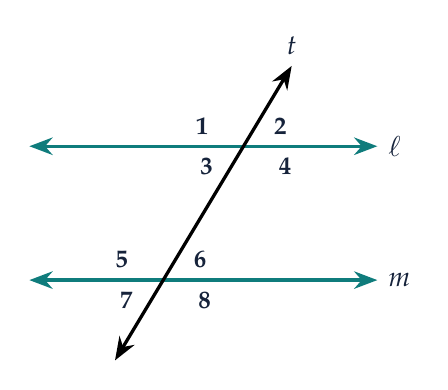
\begin{tikzpicture}[scale=0.85]\draw[very thick,fteal,{Stealth}-{Stealth}] (-2.6,1)--(2.6,1) node[right,fink]{$\ell$};\draw[very thick,fteal,{Stealth}-{Stealth}] (-2.6,-1)--(2.6,-1) node[right,fink]{$m$};\draw[very thick,{Stealth}-{Stealth}] (-1.32,-2.2)--(1.32,2.2) node[above,fink]{$t$};\node[font=\small\bfseries,text=fink] at (-0.02,1.30){1};\node[font=\small\bfseries,text=fink] at (1.15,1.30){2};\node[font=\small\bfseries,text=fink] at (0.05,0.70){3};\node[font=\small\bfseries,text=fink] at (1.22,0.70){4};\node[font=\small\bfseries,text=fink] at (-1.22,-0.70){5};\node[font=\small\bfseries,text=fink] at (-0.05,-0.70){6};\node[font=\small\bfseries,text=fink] at (-1.15,-1.30){7};\node[font=\small\bfseries,text=fink] at (0.02,-1.30){8};\end{tikzpicture}\end{column}\begin{column}{0.54\textwidth}\onslide<1->{\key{Corresponding} angles are \key{congruent}.}\par\medskip
\onslide<2->{\key{Alternate interior} and \key{alternate exterior} angles are \key{congruent}.}\par\medskip
\onslide<3->{\key{Same-side interior} angles are \key{supplementary} (add to $180^\circ$).}\par\medskip\end{column}\end{columns}
\end{frame}
\begin{frame}{The easy way to see it}
\begin{columns}[c]\begin{column}{0.44\textwidth}\centering 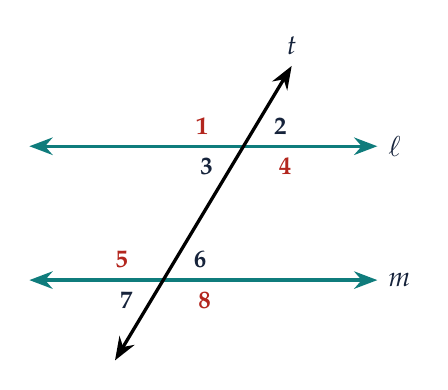
\begin{tikzpicture}[scale=0.85]\draw[very thick,fteal,{Stealth}-{Stealth}] (-2.6,1)--(2.6,1) node[right,fink]{$\ell$};\draw[very thick,fteal,{Stealth}-{Stealth}] (-2.6,-1)--(2.6,-1) node[right,fink]{$m$};\draw[very thick,{Stealth}-{Stealth}] (-1.32,-2.2)--(1.32,2.2) node[above,fink]{$t$};\node[font=\small\bfseries,text=fred] at (-0.02,1.30){1};\node[font=\small\bfseries,text=fink] at (1.15,1.30){2};\node[font=\small\bfseries,text=fink] at (0.05,0.70){3};\node[font=\small\bfseries,text=fred] at (1.22,0.70){4};\node[font=\small\bfseries,text=fred] at (-1.22,-0.70){5};\node[font=\small\bfseries,text=fink] at (-0.05,-0.70){6};\node[font=\small\bfseries,text=fink] at (-1.15,-1.30){7};\node[font=\small\bfseries,text=fred] at (0.02,-1.30){8};\end{tikzpicture}\end{column}\begin{column}{0.54\textwidth}\onslide<1->{Every angle is either \key{acute} or \key{obtuse}.}\par\medskip
\onslide<2->{Two acute angles are \key{equal}. Two obtuse angles are \key{equal}.}\par\medskip
\onslide<3->{An acute $+$ an obtuse $= \ans{180^\circ}$}\par\medskip\end{column}\end{columns}
\end{frame}
\begin{frame}{Find the angle}
\begin{columns}[c]\begin{column}{0.44\textwidth}\centering 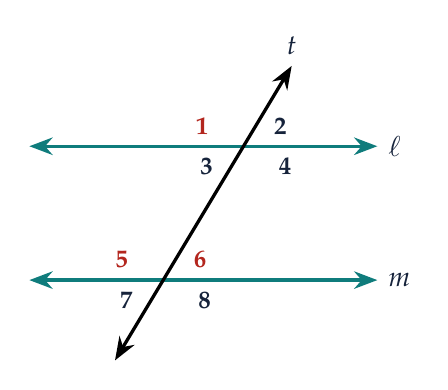
\begin{tikzpicture}[scale=0.85]\draw[very thick,fteal,{Stealth}-{Stealth}] (-2.6,1)--(2.6,1) node[right,fink]{$\ell$};\draw[very thick,fteal,{Stealth}-{Stealth}] (-2.6,-1)--(2.6,-1) node[right,fink]{$m$};\draw[very thick,{Stealth}-{Stealth}] (-1.32,-2.2)--(1.32,2.2) node[above,fink]{$t$};\node[font=\small\bfseries,text=fred] at (-0.02,1.30){1};\node[font=\small\bfseries,text=fink] at (1.15,1.30){2};\node[font=\small\bfseries,text=fink] at (0.05,0.70){3};\node[font=\small\bfseries,text=fink] at (1.22,0.70){4};\node[font=\small\bfseries,text=fred] at (-1.22,-0.70){5};\node[font=\small\bfseries,text=fred] at (-0.05,-0.70){6};\node[font=\small\bfseries,text=fink] at (-1.15,-1.30){7};\node[font=\small\bfseries,text=fink] at (0.02,-1.30){8};\end{tikzpicture}\end{column}\begin{column}{0.54\textwidth}\onslide<1->{$\ell \parallel m$, \ $m\angle 1 = 110^\circ$. \ Find $m\angle 5$ and $m\angle 6$.}\par\medskip
\onslide<2->{$\angle 1$, $\angle 5$ corresponding: \ $m\angle 5 = \ans{110^\circ}$}\par\medskip
\onslide<3->{$\angle 5$, $\angle 6$ linear pair: \ $m\angle 6 = 180 - 110 = \ans{70^\circ}$}\par\medskip\end{column}\end{columns}
\end{frame}
\begin{frame}{With algebra}
\onslide<1->{Alternate interior: $(3x + 15)^\circ$ and $(5x - 25)^\circ$}\par\medskip
\onslide<2->{Congruent: $3x + 15 = 5x - 25 \Rightarrow 40 = 2x \Rightarrow x = \ans{20}$}\par\medskip
\onslide<3->{Angle: $3(20) + 15 = \ans{75^\circ}$}\par\medskip
\end{frame}
\begin{frame}{Watch out}
\onslide<1->{\warn{Same-side interior angles are \textbf{supplementary}, not equal. Set them to add to $180^\circ$.}}\par\medskip
\end{frame}
\begin{frame}{}
\begin{yourturn}$\ell \parallel m$. Same-side interior angles are $(2x + 10)^\circ$ and $(3x - 5)^\circ$. Find $x$ and both angles.\end{yourturn}\par\medskip
\onslide<2->{$5x + 5 = 180 \Rightarrow x = \ans{35}$; \ angles \ans{80^\circ} and \ans{100^\circ}}\par\medskip
\end{frame}
\closeframe{\begin{itemize}\setlength\itemsep{8pt}
\item Parallel lines: corresponding, alternate interior, alternate exterior angles are \key{congruent}.
\item Same-side interior angles are \key{supplementary}.
\item Acute $=$ acute, obtuse $=$ obtuse, acute $+$ obtuse $= 180^\circ$.
\end{itemize}}
\end{document}
